\section{Methods}
\label{sec:methods}


Our methodology is based on implementing a closed-loop data cycle to
improve predictions from a coastal ocean model via robotic adaptive
sampling and data assimilation. The approach consists of three
fundamental steps, executed iteratively on a daily basis:

\begin{description}

\item[Model Forecast and Uncertainty Projection]: An ocean model
  provides a daily one-step forecast $\hat{\theta}(k+1, x, y)$ of a
  target oceanic variable $\theta$, along with an associated
  uncertainty field $\sigma_{\hat{\theta}}(k+1, x, y)$, where $k$
  represents the current day and $(x, y)$ denote the geographical
  coordinates. These outputs are organized into discrete spatial maps,
  $M_{\hat{\theta}}(x, y)$ and $M_{\sigma_{\hat{\theta}}}(x, y)$,
  representing, the predicted state and its uncertainty over a
  predefined grid covering the study area, respectively.

\item \textbf{Targeted Sampling}: We define areas of larger
  uncertainty predictions as areas of higher reward. Using the
  uncertainty map $M_{\sigma_{\hat{\theta}}}(x, y)$ as input, the
  targeted sampling algorithm determines the set of trajectories for
  $N$ AUVs for the next operational cycle. The goal is to maximize the
  accumulated uncertainty sampled along the vehicle trajectories.

\item \textbf{Data Collection and Assimilation}: Throughout the
  operational period, each AUV collects measurements of the target
  variable $\theta$ along its assigned path. After mission completion,
  the collected measurements are assimilated into the model using an
  appropriate data assimilation scheme. This updated model state
  serves as the new initial condition for the next forecasting cycle,
  closing the loop.

\end{description}

While previous efforts have concentrated on a form of embedded and
automated decision-making for AUV-based adaptive sampling
\cite{mcgann08a,mcgann08b,ryan10,py10,Das-2010-637,das10,olaya12,rajan12},
the trajectories in this work are generated manually, with adaptation
focused on deployment based on $M_{\sigma_{\hat{\theta}}}(x,
y)$. Here, loop closure refers to the
\emph{sample-assimilate-predict-direct} process.

\subsection{Model Forecast, Uncertainty Projection and Data Assimilation}

Sampling strategies rely on timely information about the spatial
variability of ocean properties. However, conventional numerical ocean
models are computationally intensive, and their runtime makes them
impractical for use with high spatial resolution and in near-real-time
mission planning \cite{agarwal21}. While similar assimilation cycles
could, in principle, be implemented directly within numerical models,
this would require either substantially larger computational resources
or larger temporal horizons.

As a practical alternative, we use geostatistical stochastic
sequential simulation as a computationally efficient surrogate for
short-term spatial predictions of ocean variables together with
estimates of spatial uncertainty \cite{deutsch1992}. This approach
captures the essential variability of local ocean dynamics, based on
calibrated deterministic dynamic ocean models, at a fraction of the
computational cost of numerical models, while remaining flexible
enough to rapidly assimilate new in-situ observations
\cite{Duarte2025}.  However, with this type of surrogate models we are
not explicitly considering the full-physics of the ecosystem and the
quality of the predictions directly depends on the accuracy of the
calibrated model and prediction time length. If the calibrated model
is unable to capture the true nature of the system the geostatistical
predictions will likely be inaccurate.  Equally, if there is a new
oceanographic event that is not present in the calibrated model, the
geostatistical approach will not be able to capture it.

The methodology relies on ensembles of geostatistical realizations,
each representing a state of an ocean variable field conditioned by
\emph{a priori} deterministic ocean models \cite{CMEMS2017} and direct
observations. By computing the pointwise standard deviation across the
ensemble, we obtain spatial uncertainty maps that highlight regions
where predictions are more variable and therefore potentially more
informative for robotic sampling. These maps then, serve as the basis
for identifying areas where new measurements are expected to maximize
the reduction of forecast error.

Beyond uncertainty prediction, the proposed framework also allows
direct assimilation of AUV acquired data. Data collected on a given
day are used to update the ocean variable forecast for the following
day by combining prior predictions with new measurements. The
simulation grid, in this case, includes two temporal layers: the first
containing the AUV measurements at their spatial locations and the
second corresponding to the new prediction step. With AUV sampling
denser than the grid resolution, measurements within the same grid
cell are averaged as a form of arithmetic upscaling
\cite{Duarte2025}. To incorporate spatial and temporal variability, we
apply direct sequential simulation with local means
\cite{soares2001direct}\footnote{Defined by kriging estimates and
  variances, which are conditioned to existing direct measurements and
  a spatial covariance matrix.\cite{cressie93}}, where each simulated
value is drawn from its conditional distribution, accounting for both
prior simulated values and local mean models. Doing so enables
consistent updating of the variable field while integrating both
direct AUV observations and a priori information. The ensemble of
realizations thus provides an updated ocean forecast and a
quantitative measure of uncertainty.
 
The continuity of the variable field in space and time is
characterized by variogram models fitted to long-term calibrated ocean
model data from the E.U. Copernicus Marine Service (CMS)
\cite{CMEMS2017}. For each depth layer of the deterministic model,
geostatistical simulations are performed independently using a moving
temporal window of the previous 14 days as conditioning data. This
window length was selected through comparison with the deterministic
model’s short-term evolution under similar seasonal conditions,
striking a balance between forecast stability and computational
cost. Spatial propagation occurs only horizontally within each depth
level, while vertical consistency is implicitly maintained through the
depth-specific variogram structures derived from the 3D deterministic
model.

This provides both a forecast of ocean variables being simulated, as
well as a quantitative assessment of the prediction uncertainty.  By
updating the forecasts with new in-situ measurements through
sequential assimilation, the method progressively refines the variable
field while maintaining consistency with prior model dynamics. The
resulting forecast and uncertainty maps then form the input for the
targeted sampling algorithm, guiding the allocation of AUV
trajectories towards regions of greatest expected information
gain. More details about the model, its development, and application
during the \proj experiment can be found in \cite{Duarte2025}.

\subsection{The Sampling Algorithm}

The adaptive sampling problem we pose here, is the design of vehicle
trajectories that maximize information gain
\cite{eidsvik2015,fossum18} extracted from a model-derived uncertainty
map, while satisfying operational AUV constraints. Each day, the
models provide both a forecast field and its associated uncertainty
distribution, which together define the reward landscape for the
trajectory planner. The task is to generate, for each vehicle, a tour,
that accumulates the highest possible uncertainty values. The tour is
traveled at a prescribed AUV speed while the duration is bounded above
by the assimilation period. The starting and ending point is selected
to simplify logistics for launch and recovery.

Although the underlying deterministic CMS model is fully
three-dimensional and the statistical solution also provides
predictions across multiple depth layers (as noted above), in this
work, the sampling algorithm operates on a 2-Dimensional (2D)
horizontal field derived from the 3D uncertainty structure of the
statistical solution. This field is obtained by averaging the
horizontal slices of uncertainty between the surface and 40m depth, a
depth interval chosen to represent the upper mixed layer in the study
region. Within this layer, turbulent mixing typically maintains
relatively weak vertical gradients, and most of the temperature
variability relevant for mission planning is concentrated near the
surface and the upper thermocline. Averaging across this depth range
therefore, yields a stable and physically meaningful 2D representation
of the uncertainty field.

Although the trajectory planning itself is carried out in two
dimensions, the yo-yo motion executed by the AUVs along each transect
naturally restores vertical sampling capability, compensating for the
2D approximation and enabling the acquisition of high
vertical-resolution profiles at all visited locations. This strategy
also aligns with the dominant physical and biogeochemical processes
occurring within the mixed layer, where air–sea interactions, nutrient
entrainment, and local thermal structure exert primary control on
short-term dynamics
\cite{mahadevan2016impact,behrenfeld2014resurrecting}.

The tour is formulated as a graph theoretic problem. The spatial
uncertainty map is first pre-processed to remove obstacles and
smoothed to highlight large-scale features. Candidate waypoints are
then identified from the map and used to build a weighted graph, where
nodes carry a reward proportional to their uncertainty value and edges
represent travel costs. The trajectory planning task is posed as a
tour routing problem where routes must balance the rewards obtained
from visiting nodes with associated costs of traveling between them
\cite{vidal2013,toth2014vehicle}. By solving this, the algorithm
returns a set of near-optimal trajectories that prioritize regions of
greatest uncertainty, while ensuring vehicle endurance and safety
constraints. This provides a principled way of steering autonomous
platforms toward the most informative sampling locations, forming a
key component in the daily cycle of forecast, sampling, and
assimilation. Additional insights into the algorithm and its
deployment during \proj are reported elsewhere in
\cite{bernacchi2025}.

\subsection{Operations and Data Collection}

\begin{figure}
    \centering
    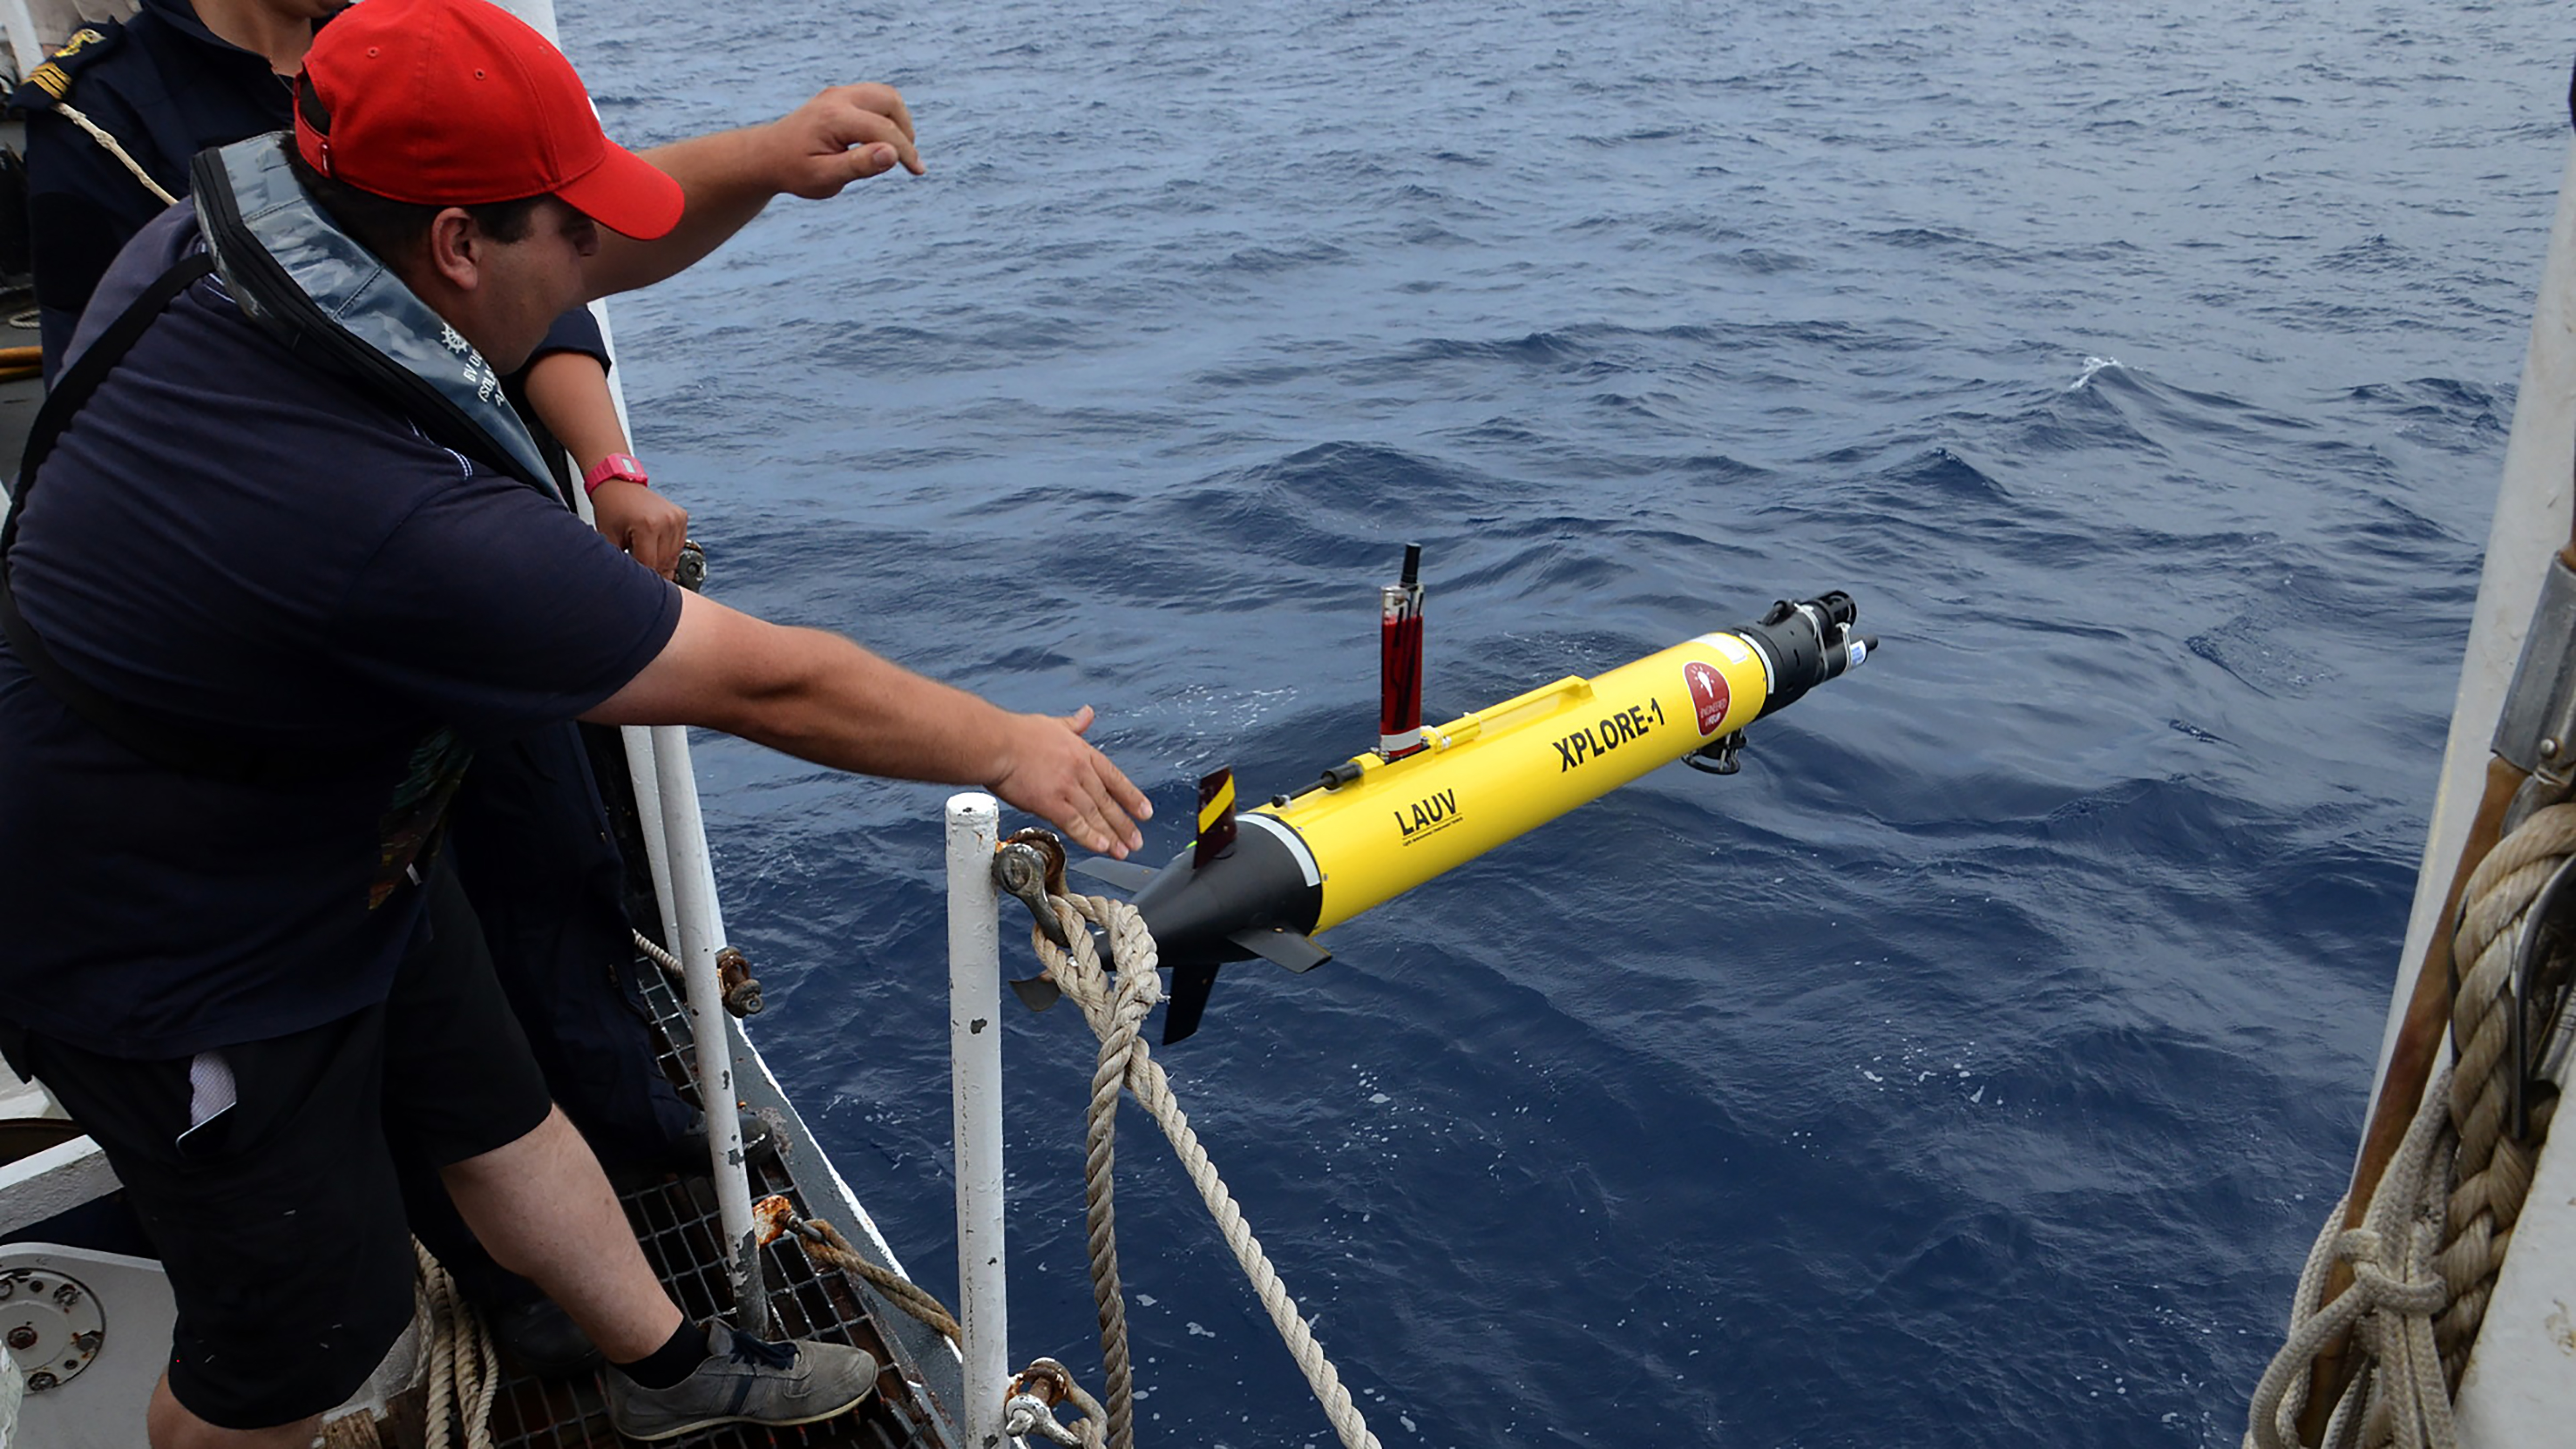
\includegraphics[width=.7\linewidth]{fig/DSC_8342.JPG}
    \caption{Multiple Light Autonomous Underwater Vehicles such as
      the one shown above, were used in \proje. This low-cost platform
      designed at the University of Porto has demonstrated its
      robustness and integration to a number of oceanographic sensors
      and comes with a sizable open source command/control software.}
    \label{fig:lauvs}
\end{figure}

The in-situ data collection process involved three upper water-column
Light Autonomous Underwater Vehicles (LAUV) (XP2, XP3 and
XP5)\footnote{We will refer to these specific vehicles across the
  three day period given the diversity and specificity of their
  operating environments and measurements.} which performed targeted
sampling missions with durations of up to 60 hours over the \naz
Canyon region, with all vehicles sampling the upper 100m of the water
column. These vehicles designed and developed in-house at the
University of Porto \cite{sousa2012lauv} came equipped with a range of
sensors including a CTD (Fig. \ref{fig:lauvs}) along with WiFi and
Iridium satellite communications; the CTDs mounted on the AUVs were
cross-calibrated to ensure consistency. In addition to the hardware
involved, an extensive suite of mature mission planning and
command/control tools were used -- discussion of these is outside the
scope of the paper and can be referenced in
\cite{dias2005neptus,seacons10,toolchain2012,pinto2013lsts,Ferreira2018}.

The experiment had a small human and support vessel footprint,
demonstrating significant cost reduction in comparison to traditional
ship-based methods while measuring at higher spatial and temporal
resolution. Operations were conducted continuously by pairs of
operators working 6 hour shifts based in Porto as well as in \naz --
the intervention of small boats was limited to the launch and recovery
of AUVs, that operated unattended.


Challenging meteorological and ocean conditions constrained the number
of consecutive iterations of the
\emph{sample-assimilate-predict-direct} loop to a three-day sequence
of experiments (29\textsuperscript{th} – 31\textsuperscript{st}
October, 2025) (Fig. \ref{fig:scheme}). For the sake of clarity, the
presentation of the workflow and assimilation loop is focused only on
temperature measurements. As a consequence this work is univariate in
showing the impact of assimilated model-driven exploration. We believe
that results in Sec \ref{sec:results} are general enough to apply to
other critical oceanographic variables which would be modeled
similarly. The analysis in this work therefore, ultimately aims to
quantify the impact of assimilating AUV-acquired temperature data on
the predictive performance of the statistical model and to assess the
operational feasibility of the data cycle approach in a coastal
setting.

Each experimental day followed a structured cycle involving: (i) the
generation of a statistical model forecast and its associated
uncertainty field based on the CMS data available up to the previous
day \cite{sotillo2021}; (ii) the execution of the target sampling
algorithm to plan the next day missions; and (iii) in-situ data
collection by AUVs following the algorithmically determined tours. The
data collected within the previous day were subsequently assimilated
into the statistical model to produce updated forecasts, enabling
comparisons between forecasts with and without data assimilation.

% \begin{wrapfigure}{!h}{4.4in}
%   \centering
%   \includegraphics[scale=0.38]{fig/scheme.png}
%   \caption{Three-day sequence
%     (29\textsuperscript{th}–-31\textsuperscript{st} October 2025) of
%     the \emph{sample-–assimilate–-predict-–direct} loop in the \proj
%     experiment. Each cycle integrated CMS derived statistical model
%     prediction, targeted sampling, AUV data acquisition and subsequent
%     assimilation for prediction for the following day.}
%   \label{fig:scheme}
% \end{wrapfigure}


\begin{figure}[!t]
  \centering
  \includegraphics[scale=0.3]{fig/scheme.png}
  \caption{Three-day sequence
    (29\textsuperscript{th} - 31\textsuperscript{st} October 2025) of
    the \emph{sample-–assimilate–-predict-–direct} loop in the \proj
    experiment. Each cycle integrated CMS derived statistical model
    prediction, targeted sampling, AUV data acquisition and subsequent
    assimilation for prediction for the following day.}
  \label{fig:scheme}
\end{figure}

\subsubsection{A Multi-scenario framework}

Given challenges related to weather, assimilation and model
prediction, and multiple AUVs, a number of scenario solutions
contribute to the final solution set. These scenarios, labelled
\textbf{A} through \textbf{D} (and their corresponding assimilation
variants) are summarised in Table \ref{table:scenarios}. The table
provides a compact, color-coded overview of all configurations (used
in Figs. \ref{fig:rms_ABB1} and \ref{fig:rms}), including forecast
dates, prior CMS fields, and the specific AUV datasets assimilated at
each stage.

On 29\textsuperscript{th} October, the statistical model produced the
initial forecast solution (\textbf{A}), which was used to plan the
mission executed by XP2 (Fig. \ref{fig:scheme}). The resulting data
was assimilated offline to produce an updated statistical model
solution (\textbf{B1}) for 30\textsuperscript{th} October. Although
operational real-time assimilation was initially planned, logistical
constraints prevented its implementation; consequently, all
assimilation was performed offline after AUV mission completion. The
targeted sampling algorithm, therefore, relied on statistical
forecasts \emph{without} assimilation (\textbf{B}), using pre-existing
data as input for daily mission planning. This limitation is not
expected to have significantly affected the experimental outcomes, as
the operational area was spatially compact and the predicted
variability field remained consistent between consecutive
days\footnote{In future implementations, on-board or near-real-time
  assimilation would need to be considered to fully exploit the
  adaptive potential of the framework}.

For 31\textsuperscript{st} October, multiple assimilation
configurations were tested to quantify how the information collected
on previous days could influence short-term predictive
skill. Measurements from XP3 and XP5 on 30\textsuperscript{st} October
were assimilated offline to generate scenarios
\textbf{C1}-–\textbf{C4}, complementing the non-assimilated reference
case \textbf{C}. These cases progressively integrate different subsets
of AUV observations, ranging from XP2-only data (\textbf{C1}) to the
full multi-vehicle dataset from 29\textsuperscript{st} to
30\textsuperscript{th} October (\textbf{C4}).

A parallel set of scenarios (\textbf{D} and \textbf{D1} - \textbf{D4})
was generated to evaluate the sensitivity of the statistical model to
the choice of prior CMS fields. The \textbf{D}-series uses CMS data
available only up to 29\textsuperscript{st} October, thus representing
a less favorable initial state, and applies the same assimilation
configurations as in the \textbf{C}-series. This dual-series approach
enables a controlled comparison of how data assimilation interacts
with differences in model initialization.

Model performance was evaluated by comparing predicted and observed
temperature data along the AUV trajectories using Root Mean Square
Error (RMSE) as the performance metric for 31\textsuperscript{st}
October.

\begin{table}[]
  \centering \resizebox{\columnwidth}{!}{%
    \footnotesize{
\begin{tabular}{cccc}
\hline
\textbf{Scenario}                  & \textbf{Forecast date} & \textbf{CMS prior data up to} & \textbf{Assimilated AUV datasets} \\ \hline
{\color[HTML]{3531FF} \textbf{A}}  & 29 Oct                 & 28 Oct                        & None (baseline)                   \\ \hline
{\color[HTML]{9A0000} \textbf{B}}  & 30 Oct                 & 29 Oct                        & None (baseline)                   \\
{\color[HTML]{FFCB2F} \textbf{B1}} & 30 Oct                 & 29 Oct                        & XP2 (29 Oct)                      \\ \hline
{\color[HTML]{3531FF} \textbf{C}}  & 31 Oct                 & 30 Oct                        & None (baseline)                   \\
{\color[HTML]{9A0000} \textbf{C1}} & 31 Oct                 & 30 Oct                        & XP2 (29 Oct)                      \\
{\color[HTML]{FFCB2F} \textbf{C2}} & 31 Oct                 & 30 Oct                        & XP2 (29 Oct), XP5 (30 Oct)        \\
{\color[HTML]{6200C9} \textbf{C3}} & 31 Oct                 & 30 Oct                        & XP5 (30 Oct)                      \\
{\color[HTML]{009901} \textbf{C4}} & 31 Oct                 & 30 Oct                        & XP2, XP3, XP5 (29–30 Oct)         \\ \hline
{\color[HTML]{3531FF} \textbf{D}}  & 31 Oct                 & 29 Oct                        & None (baseline)                   \\
{\color[HTML]{9A0000} \textbf{D1}} & 31 Oct                 & 29 Oct                        & XP2 (29 Oct)                      \\
{\color[HTML]{FFCB2F} \textbf{D2}} & 31 Oct                 & 29 Oct                        & XP2 (29 Oct), XP5 (30 Oct)        \\
{\color[HTML]{6200C9} \textbf{D3}} & 31 Oct                 & 29 Oct                        & XP5 (30 Oct)                      \\
{\color[HTML]{009901} \textbf{D4}} & 31 Oct                 & 29 Oct                        & XP2, XP3, XP5 (29–30 Oct)         \\ \hline
\end{tabular}%
}}
\caption{Summary of scenarios and assimilation configurations. The
  color codes are referred to in Figs. \ref{fig:rms_ABB1} and
  \ref{fig:rms} to disambiguate RMSE plots.}
\label{table:scenarios}
\end{table}


% \begin{figure}
%     \centering
%     %\includegraphics[width=.7\linewidth]{fig/temperatureprofiles.png}
%     \caption{INSERT schematic about the 3-day loop}
%     \label{fig:temperatureprofiles}
% \end{figure}

% PLEASE CHECK CAPTION OF FIGURE 3 - I have done this sequentially, except for this mod
%   \label{fig:loop-closure} 
